\chapter{Overview of Supervised Learning}
\begin{exer}
    Suppose that each of $K$-classes has an associated target $t_k$, which is a vector of all zeroes, except a one in the $k$-th position.  Show that classifying the largest element of $\hat y$ amounts to choosing the closest target, $\min_k \| t_k - \hat y \|$ if the elements of $\hat y$ sum to one. 
\end{exer}

\begin{proof}
    The assertion is equivalent to showing that \[
    \argmax_i \hat y_i = \argmin_k \| t_k - \hat y \| = \argmin_k \|\hat y - t_k \|^2
\] by monotonicity of $x \mapsto x^2$ and symmetry of the norm.  

WLOG, let $\| \cdot \|$ be the Euclidean norm $\| \cdot \|_2$.  Let $k = \argmax_i \hat y_i$, with $\hat y_k = \max y_i$.  Note that then $\hat y_k \geq \frac{1}{K}$, since $\sum \hat y_i = 1$.   

Then for any $k' \neq k$ (note that $y_{k'} \leq y_k$), we have \begin{align*}
    \| y - t_{k'} \|_2^2 - \| y - t_k \|_2^2 &= y_k^2 + \left(y_{k'} - 1 \right)^2 - \left( y_{k'}^2 + \left(y_k - 1 \right)^2 \right) \\
    &= 2 \left(y_k - y_{k'}\right) \\
    &\geq 0
\end{align*} since $y_{k'} \leq y_k$ by assumption.

Thus we must have \[
    \argmin_k \| t_k - \hat y \| = \argmax_i \hat y_i
\] as required.    
\end{proof}

\begin{exer}
    Show how to compute the Bayes decision boundary for the simulation example in Figure 2.5.
\end{exer}

\begin{proof}
    The Bayes classifier is \[
        \hat G(X) = \argmax_{g \in \mathcal G} P(g | X = x ).
    \] In our two-class example $\textsc{orange}$ and $\textsc{blue}$, the decision boundary is the set where \[
        P(g=\textsc{blue} | X = x) = P(g =\textsc{orange} | X = x) = \frac{1}{2}.
    \]  
    
    By the Bayes rule, this is equivalent to the set of points where \[
        P(X = x | g = \textsc{blue}) P(g = \textsc{blue}) = P(X = x | g = \textsc{orange}) P(g = \textsc{orange})
    \] And since we know $P(g)$ and $P(X=x|g)$, the decision boundary can be calculated.
\end{proof}

\begin{exer}
    Derive equation (2.24)
\end{exer}

\begin{proof}
    TODO
\end{proof}
    
\begin{exer}
    Consider $N$ data points uniformly distributed in a $p$-dimensional unit ball centered at the origin.  Show the the median distance from the origin to the closest data point is given by \[
        d(p, N) = \left(1-\left(\frac{1}{2}\right)^{1/N}\right)^{1/p}
    \] 
\end{exer}
\begin{proof}
    Let $r$ be the median distance from the origin to the closest data point.  Then \[
        P(\text{All $N$ points are further than $r$ from the origin}) = \frac{1}{2}
    \] by definition of the median.

    Since the points $x_i$ are independently distributed, this implies that \[
        \frac{1}{2} = \prod_{i=1}^N P(\|x_i\| > r)
    \] and as the points $x_i$ are uniformly distributed in the unit ball, we have that \begin{align*}
        P(\| x_i \| > r) &= 1 - P(\| x_i \| \leq r) \\
                         &= 1 - \frac{Kr^p}{K} \\
                         &= 1 - r^p
    \end{align*}  Putting these together, we obtain that \[
        \frac{1}{2} = \left(1-r^p \right)^{N}
    \] and solving for $r$, we have \[
        r = \left(1-\left(\frac{1}{2}\right)^{1/N}\right)^{1/p}
    \]
\end{proof}

\begin{exer}
    Consider inputs drawn from a spherical multivariate-normal distribution $X \sim N(0,\mathbf{1}_p)$. The squared distance from any sample point to the origin has a $\chi^2_p$ distribution with mean $p$. Consider a prediction point $x_0$ drawn from this distribution, and let $a = \frac{x_0}{\| x_0\|}$ be an associated unit vector. Let $z_i = a^T x_i$ be the projection of each of the training points on this direction.
    Show that the $z_i$ are distributed $N(0,1)$ with expected squared distance from the origin 1, while the target point has expected squared distance $p$ from the origin.
    Hence for $p = 10$, a randomly drawn test point is about 3.1 standard deviations from the origin, while all the training points are on average one standard deviation along direction a. So most prediction points see themselves as lying on the edge of the training set.
\end{exer}

\begin{proof}
    Let $z_i = a^T x_i = \frac{x_0^T}{\| x_0 \|} x_i$.  Then $z_i$ is a linear combination of $N(0,1)$ random variables, and hence normal, with expectation zero and variance \[ 
        \text{Var}(z_i) = \| a^T \|^2 \text{Var}(x_i) = \text{Var}(x_i) = 1
    \] as the vector $a$ has unit length and $x_i \sim N(0, 1)$.
    
    For each target point $x_i$, the squared distance from the origin is a $\chi^2_p$ distribution with mean $p$, as required.  
\end{proof}

\begin{exer}
    \begin{enumerate}[(a)]
        \item Derive equation (2.27) in the notes.
        \item Derive equation (2.28) in the notes.
    \end{enumerate}
\end{exer}

\begin{proof}
    \begin{enumerate}[(i)]
        \item We have \begin{align*}
            EPE(x_0) &= E_{y_0 | x_0} E_{\mathcal{T}}(y_0 - \hat y_0)^2 \\
                     &= \text{Var}(y_0|x_0) + E_{\mathcal T}[\hat y_0 - E_{\mathcal T} \hat y_0]^2 + [E_{\mathcal T} - x_0^T \beta]^2 \\
                     &= \text{Var}(y_0 | x_0) + \text{Var}_\mathcal{T}(\hat y_0) + \text{Bias}^2(\hat y_0).
        \end{align*}  We now treat each term individually.  Since the estimator is unbiased, we have that the third term is zero.  Since $y_0 = x_0^T \beta + \epsilon$ with $\epsilon$ an $N(0,\sigma^2)$ random variable, we must have $\text{Var}(y_0|x_0) = \sigma^2$.  

        The middle term is more difficult.  First, note that we have \begin{align*}
            \text{Var}_{\mathcal T}(\hat y_0) &= \text{Var}_{\mathcal T}(x_0^T \hat \beta) \\
                    &= x_0^T \text{Var}_{\mathcal T}(\hat \beta) x_0 \\
                    &= E_{\mathcal T} x_0^T \sigma^2 (\mathbf{X}^T \mathbf{X})^{-1} x_0
            \end{align*} by conditioning (3.8) on $\mathcal T$.
        \item TODO
    \end{enumerate}
\end{proof}

\begin{exer}
    Consider a regression problem with inputs $x_i$ and outputs $y_i$, and a parameterized model $f_\theta(x)$ to be fit with least squares.  Show that if there are observations with \emph{tied} or \emph{identical} values of $x$, then the fit can be obtained from a reduced weighted least squares problem.
\end{exer}

\begin{proof}
    This is relatively simple.  WLOG, assume that $x_1 = x_2$, and all other observations are unique.  Then our RSS function in the general least-squares estimation is \[
        RSS(\theta) = \sum_{i=1}^N \left(y_i - f_\theta(x_i) \right)^2 = \sum_{i=2}^N w_i \left(y_i - f_\theta(x_i) \right)^2 
    \] where \[
        w_i = \begin{cases}
            2 & i = 2 \\
            1 & \text{otherwise}
        \end{cases}
    \]
    Thus we have converted our least squares estimation into a reduced weighted least squares estimation.  This minimal example can be easily generalised.
\end{proof}

\begin{exer}
    Suppose that we have a sample of $N$ pairs $x_i, y_i$, drawn IID from the distribution such that \begin{align*}
        x_i \sim h(x), \\
        y_i = f(x_i) + \epsilon_i, \\
        E(\epsilon_i) = 0, \\
        \text{Var}(\epsilon_i) = \sigma^2.
    \end{align*}
    
    We construct an estimator for $f$ linear in the $y_i$, \[
        \hat f(x_0) = \sum_{i=1}^N \ell_i(x_0; \mathcal X) y_i
    \] where the weights $\ell_i(x_0; X)$ do not depend on the $y_i$, but do depend on the training sequence $x_i$ denoted by $\mathcal X$.  
    \begin{enumerate}[(a)]
        \item Show that the linear regression and $k$-nearest-neighbour regression are members of this class of estimators.  Describe explicitly the weights $\ell_i(x_0; \mathcal X)$ in each of these cases.
        \item Decompose the conditional mean-squared error \[
            E_{\mathcal Y | \mathcal X} \left( f(x_0) - \hat f(x_0) \right)^2
        \] into a conditional squared bias and a conditional variance component.  $\mathcal Y$ represents the entire training sequence of $y_i$.
        \item Decompose the (unconditional) MSE \[
            E_{\mathcal Y, \mathcal X}\left(f(x_0) - \hat f(x_0) \right)^2
        \] into a squared bias and a variance component.
        \item Establish a relationship between the square biases and variances in the above two cases.
    \end{enumerate}
\end{exer}

\begin{proof}
    \begin{enumerate}[(a)]
        \item Recall that the estimator for $f$ in the linear regression case is given by \[
            \hat f(x_0) = x_0^T \beta 
        \] where $\beta = (X^T X)^{-1} X^T y$.  Then we can simply write \[
            \hat f(x_0) = \sum_{i=1}^N \left( x_0^T (X^T X)^{-1} X^T \right)_i y_i.
        \]  Hence \[
            \ell_i(x_0; \mathcal X) = \left( x_0^T (X^T X)^{-1} X^T \right)_i.
        \]
        
        In the $k$-nearest-neighbour representation, we have \[
            \hat f(x_0) = \sum_{i=1}^N \frac{y_i}{k} \mathbf{1}_{x_i \in N_k(x_0)}
        \] where $N_k(x_0)$ represents the set of $k$-nearest-neighbours of $x_0$.  Clearly, \[
            \ell_i(x_0; \mathcal X) = \frac{1}{k} \mathbf{1}_{x_i \in N_k(x_0)}
        \]
        \item TODO
        \item TODO
        \item TODO
    \end{enumerate}
\end{proof}

\begin{exer}
    Compare the classification performance of linear regression and $k$-nearest neighbour classification on the \texttt{zipcode} data.  In particular, consider on the \texttt{2}'s and \texttt{3}'s, and $k = 1, 3, 5, 7, 15$.  Show both the training and test error for each choice.
\end{exer}

\begin{proof}    
Our implementation in R and graphs are attached.

\clearpage
\lstinputlisting{./ElemStatLearnCode/src/exercise_2_8.R}

\clearpage
\begin{figure}
\centering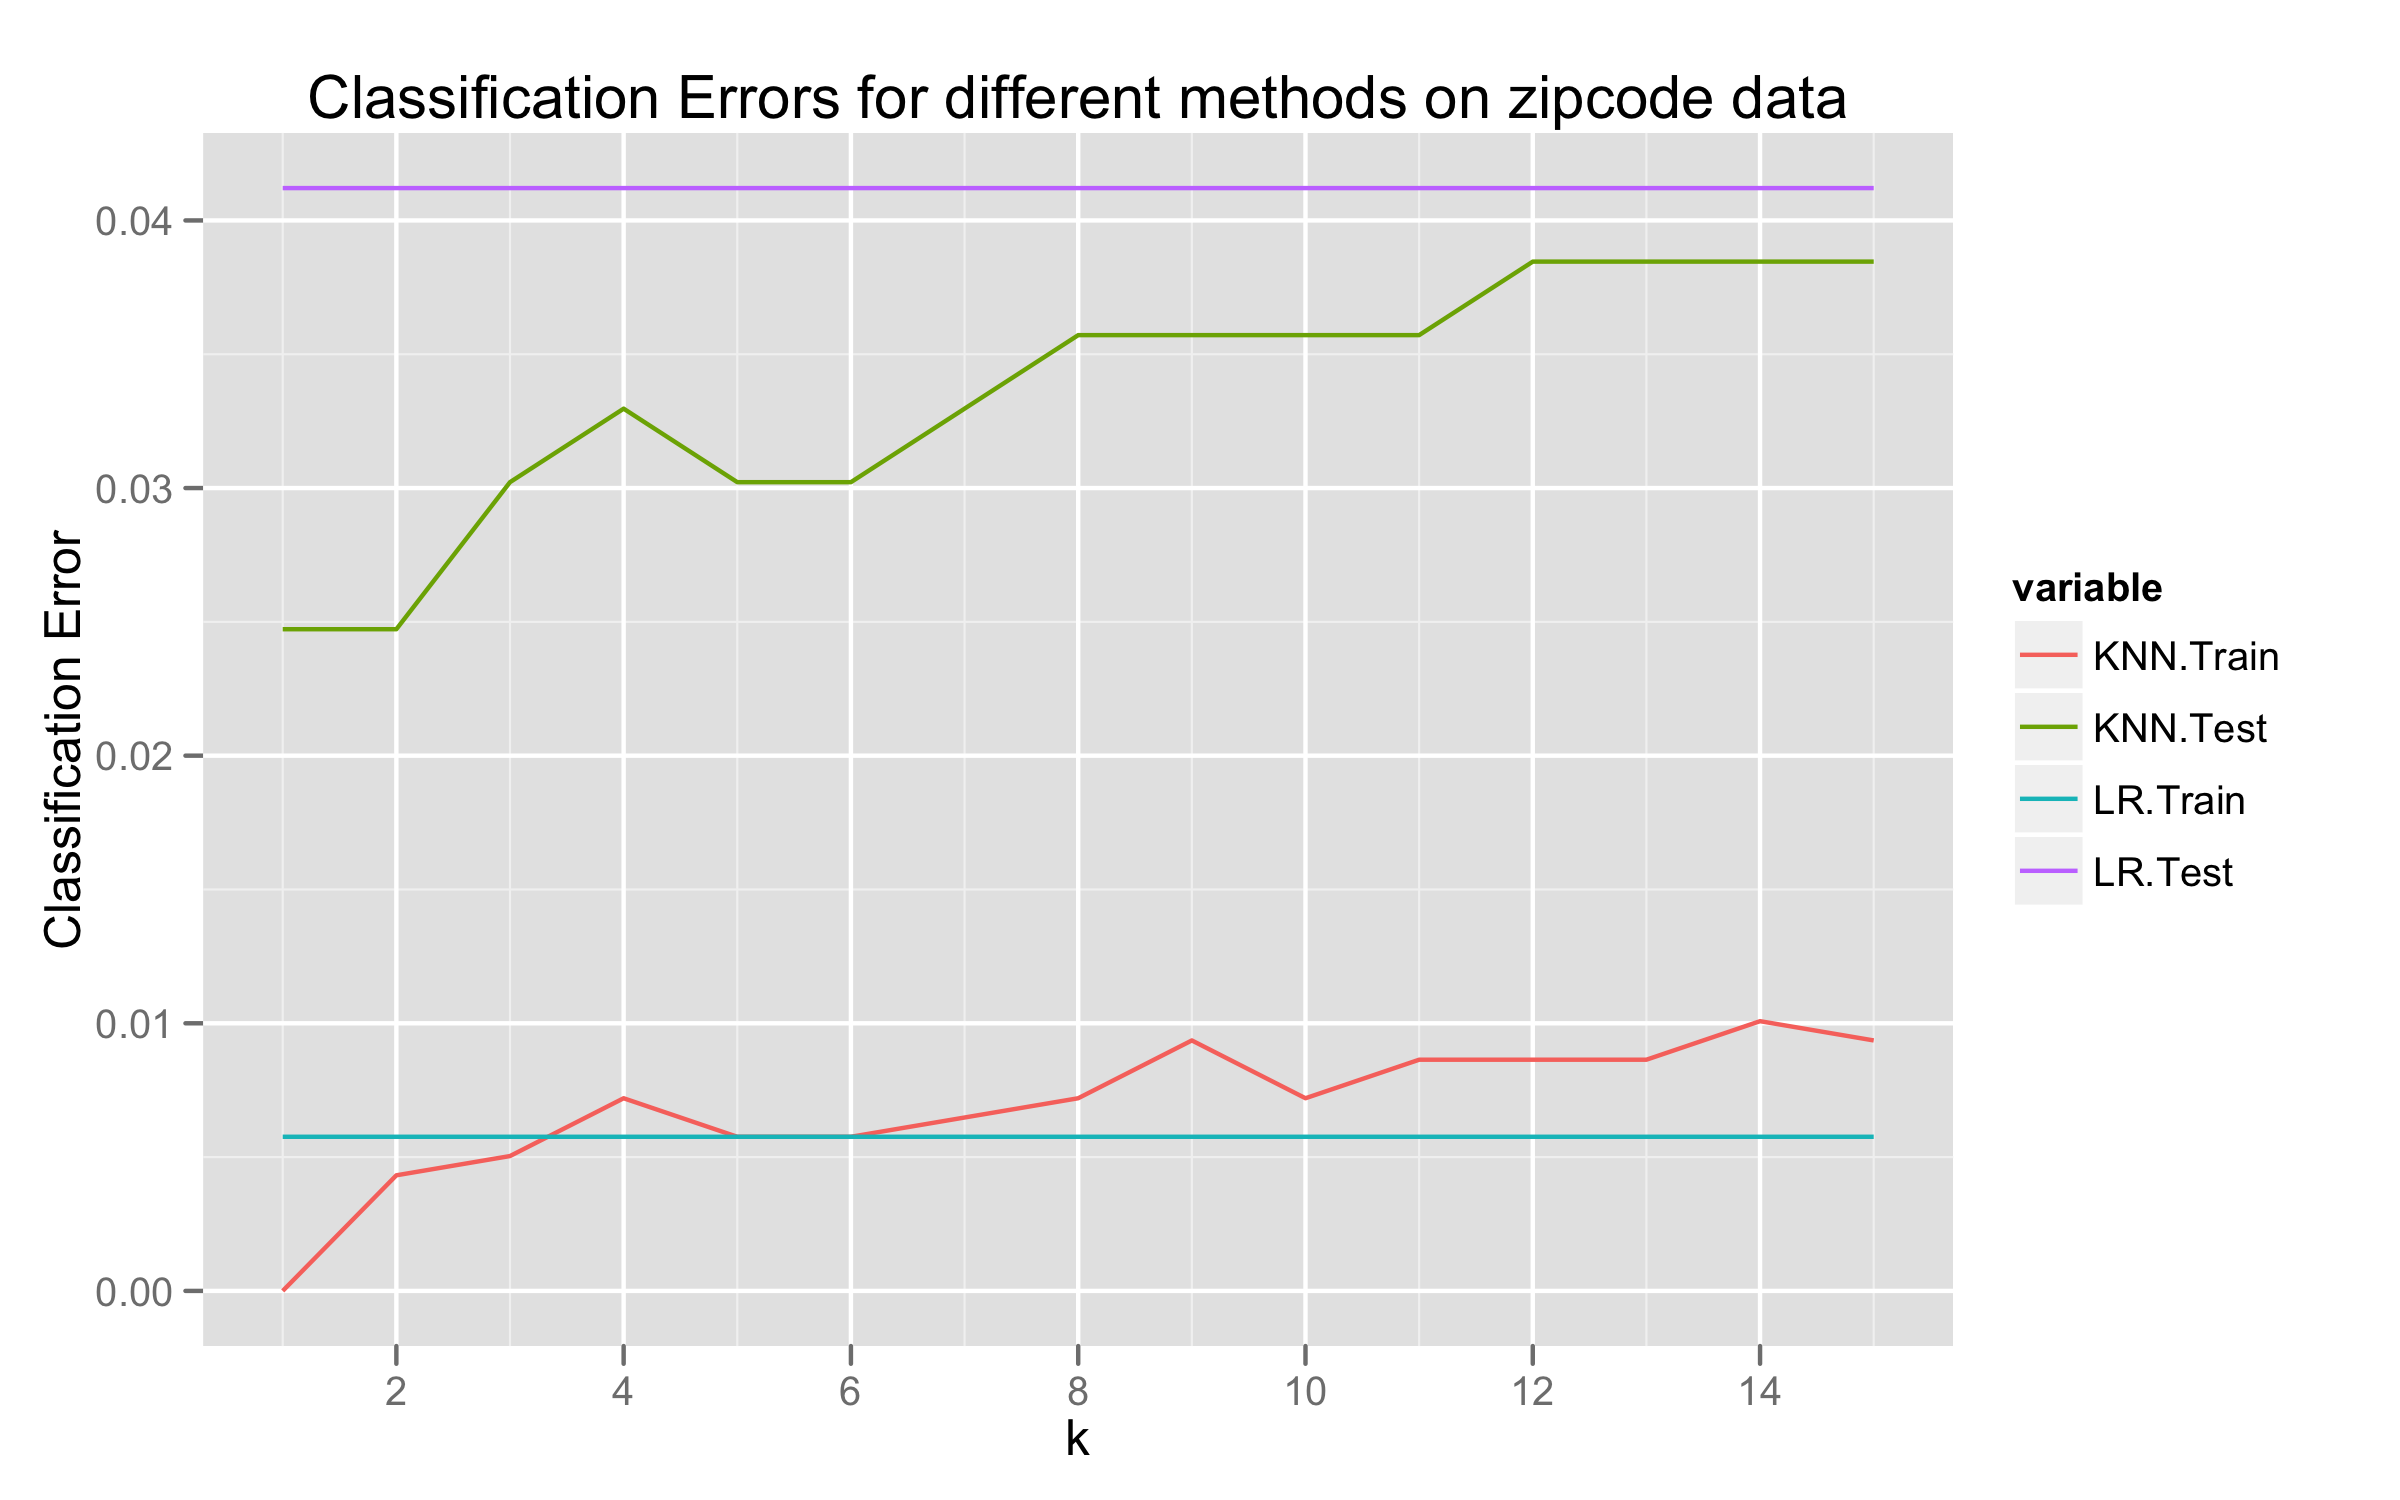
\includegraphics[width=\textwidth]{./ElemStatLearnCode/graphs/exercise_2_8.pdf}
\end{figure}

\end{proof}

\begin{exer}
    Consider a linear regression model with $p$ parameters, fitted by OLS to a set of trainig data $(x_i, y_i)_{1 \leq i \leq N}$ drawn at random from a population.  Let $\hat \beta$ be the least squares estimate.  Suppose we have some test data $(\tilde x_i, \tilde y_i)_{1 \leq i \leq M}$ drawn at random from the same population as the training data.
    
    If $R_{tr}(\beta) = \frac{1}{N} \sum_{i=1}^N \left(y_i \beta^T x_i \right)^2$ and $R_{te}(\beta) = \frac{1}{M} \sum_{i=1}^M \left( \tilde y_i - \beta^T \tilde x_i \right)^2$, prove that \[
        E(R_{tr}(\hat \beta)) \leq E(R_{te}(\hat \beta))
    \] where the expectation is over all that is random in each expression.
\end{exer}
